\documentclass[a4j, twocolumn, 10pt,pdflatex,ja=standard]{bxjsarticle}
\usepackage{graphicx}
\usepackage{amsmath,amssymb,bm}
\setlength{\headheight}{0mm}
\setlength{\headsep}{0mm}
\setlength{\footskip}{0mm}
%\setlength{\topmargin}{-30mm}
\setlength{\topmargin}{-14mm}
\setlength{\oddsidemargin}{-8mm}
\setlength{\evensidemargin}{-8mm}
\setlength{\textheight}{275mm}
\setlength{\textwidth}{176mm}
%\renewcommand{\baselinestretch}{0.85}
%\renewcommand{\refname}{\large 参�??��献}

\renewcommand{\figurename}{図}
\renewcommand{\tablename}{表}
\def \figref  #1{\figurename\ref{#1}}
\def \tabref  #1{\tablename\ref{#1}}
\def \equref  #1{\ref{#1})}

\makeatletter
\renewcommand\maketitle{
  \ifnum \col@number=\@ne \@maketitle
  \else \twocolumn[
    \vspace{-16mm}
    \@maketitle
  ]
  \fi
 }
\makeatother

\pagestyle{empty}

\title{{\small $<$2023 年度 夏学期輪講 ミニサーベイ論文第一稿$>$}\\
       {\Large ロボット制御分野における強化学習の動向調査}\vspace{-4mm}}
       \author{{\normalsize 指導教員: 國吉康夫教授\\機械情報学科03-220283 西宮直志}\vspace{-4mm}}
\date{\small 令和 5 年 6 月 19 日}
%\date{\small \today}

\usepackage{titlesec}
\titleformat*{\section}{\Large\bfseries}
\titleformat*{\subsection}{\normalsize\bfseries}


\begin{document}
\maketitle \thispagestyle{empty}
\normalsize
\vspace{-8mm}

\section{はじめに}

従来のロボット制御技術は、特定の要件に合わせたプログラムやシステムによって制御され、柔軟性や適応性に課題があった. しかし、機械学習アルゴリズムの急速な発展により、ロボット制御において環境を柔軟に理解し、より適切な行動を選択することが可能となり、様々なタスクの解決に驚くべき成果が得られている. 

本稿では、ロボティクスの制御技術に使用される機械学習アルゴリズムに関する包括的な調査を提供する. ロボットは、知覚情報に基づいて適切な行動を選択する必要がある. 機械学習アルゴリズムは、制御システムの設計や最適化において重要な役割を果たしている. また、モデル予測制御や最適制御においても、機械学習アルゴリズムが効果的に活用されている. 強化学習は、環境のモデルを使用したモデルベースの学習と、環境モデルを使用しないモデルフリーの学習に分けられるが、本稿ではモデルフリーのアプローチに焦点を当て、最後に、現在のロボティクス分野における強化学習の問題にも触れる. 

\section{価値ベースの強化学習}

価値ベースの強化学習は、行動価値関数を使用して最適な行動の評価と選択を行う手法である. 以下に、いくつかの代表的な価値ベースの強化学習アルゴリズムを述べる. 

Q学習は、強化学習の一種であり、エージェントが環境との相互作用を通じて最適な行動を学習するための手法である. しかし、状態や行動の空間が大きい場合や連続的な状態空間の場合には、テーブルを使用することが困難になるなどの問題が生じたため、DQN(Deep Q-Network)\cite{dqn}では深層学習を用いて価値関数であるQ関数を近似する手法が提案された. DQNの特徴的な要素は、Experience Replay(経験再生)と呼ばれるテクニックである. 経験再生ではエージェントがデータサンプルを記録し、そこからミニバッチ学習を行うことにより学習の効率と安定性が向上した. Zhang Fらはカメラ画像をもとにDQNを用いて3関節ロボットマニピュレータを動かすことに成功したが、カメラの位置等の画像の差異や動作の堅牢性に問題があった\cite{dqnrobot}. 

NAF (Normalized Advantage Functions) \cite{naf} は、強化学習において連続的な行動空間での制御を扱うための手法である. NAFは連続的な制御タスクにおいて効果的な行動選択を実現するための新規性を持っており、ドローンのモータのコントローラに使われた研究では、制御入力の滑らかさが向上し電力使用量を8割抑えることに成功した\cite{NAFdrone}. 

\begin{figure}[htbp]
 \begin{center}
 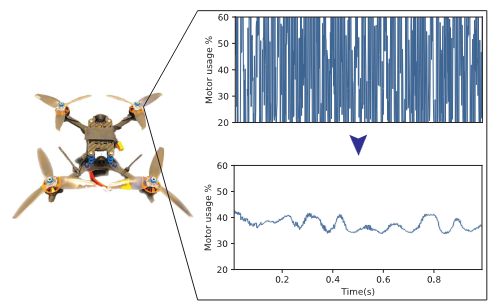
\includegraphics[height=4cm]{./figure/nafdrone.png}
 \caption{NAFを用いたドローンの制御で制御入力を滑らかにすることに成功した.}
 \label{fig:mri}
 \end{center}
\end{figure}
\vspace{-9mm}


他にもDDQN\cite{ddqn}や、UAVやテンセグリティなどの制御で効果を上げているGPS\cite{gps}、Gorilla\cite{gorilla}などがあるが、近年は以下のようなモデルが提案され、高いパフォーマンスを達成している.
\begin{figure}[htbp]
  \begin{center}
  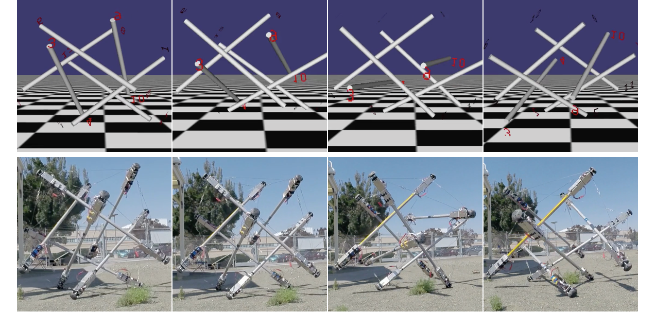
\includegraphics[height=4cm]{./figure/tensegriti.png}
  \caption{GPSを用いてテンセグリティの回転モーションを生成する様子\cite{gps}}
  \label{fig:mri}
  \end{center}
\end{figure}
\vspace{-9mm}

Rainbow\cite{rainbow}は、強化学習において重要な役割を果たすいくつかの手法を組み合わせた統合的なアルゴリズムである. これにはDQNや、優先度ベースの経験再生、分散学習、デュエルネットワーク、二重Q学習などが含まれており. サンプル効率性や安定性の向上に貢献した. 

\begin{figure}[htbp]
  \begin{center}
  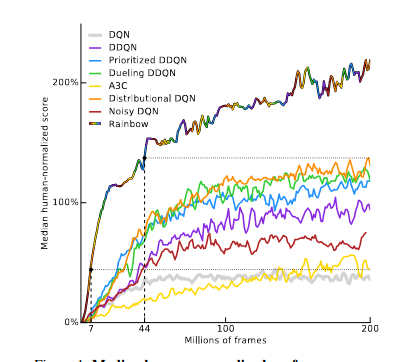
\includegraphics[height=5.5cm]{./figure/rainbow-result.png}
  \caption{Atariゲームにおける人間に対するパフォーマンス比較. Rainbowが高い精度を示している}
  \label{fig:mri}
  \end{center}
\end{figure}

\newpage


また、近年は R2d2\cite{r2d2}やそれを改良したR2D3\cite{r2d3}のようなアーキテクチャが提案されている。これはQ値計算時により効率的に時系列を扱うことで、より高いパフォーマンスを達成している.
\begin{figure}[htbp]
 \begin{center}
 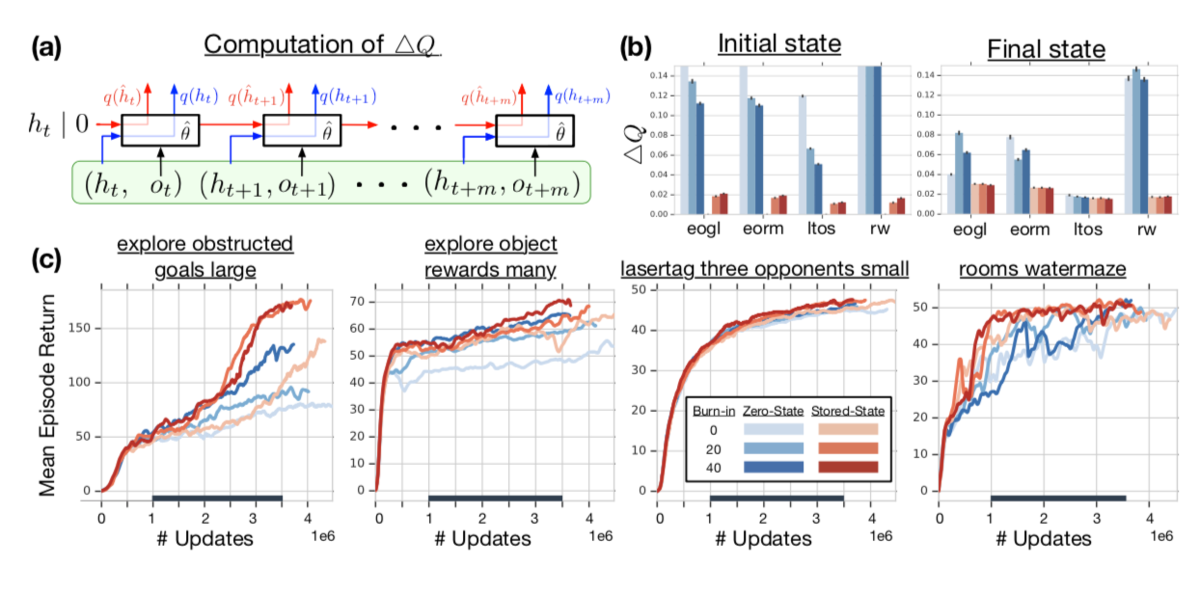
\includegraphics[height=4cm]{./figure/r2d2.png}
 \caption{R2d2}
 \label{fig:mri}
 \end{center}
\end{figure}
\vspace{-9mm}

Agent57\cite{agent57}は、Atari 2600のゲームをプレイするエージェントを訓練するための強化学習アルゴリズムであり. 深層強化学習と転移学習を組み合わせて使用し、複数のタスクを学習することで汎化性能を向上させた. また、Agent57は探索と利用のトレードオフを管理するためのmeta controllerを導入し、高いパフォーマンスを達成した. 


\section{方策ベースまたは方策+価値ベース}
方策勾配法(Policy Gradient)は、強化学習における方策(行動選択の戦略)を直接最適化する手法である. この手法では、エージェントが環境との相互作用を通じて得られる報酬を最大化するために、方策のパラメータを更新する. 

Actor-Critic\cite{ac} は、方策勾配法の一種であり、方策(Actor)と価値関数(Critic)の2つのモデルを組み合わせて学習を行う. Actorは方策モデルであり、状態に対して行動を生成する. Criticは状態価値関数や行動価値関数などの価値関数モデルであり、エージェントの行動の価値を評価する. Actorは方策の改善を目指して方策勾配法によって学習し、Criticは方策の評価や学習の補助として使用される. 

Soft Actor Critic(SAC)\cite{sac} は、Actor-Critic手法の一種であり、特に連続的な行動空間での強化学習において効果的とわかった. SACは、最適化の際にエントロピー項を利用することで、探索と利用のトレードオフを調整する. エントロピー項は方策の確率分布のランダム性を保持し、探索を促進する. SACは、高いパフォーマンスと安定性を実現し、データ効率性を向上させることができる. 


\section{今後の発展と課題}

\subsection{階層的なタスクに対する対処}
現在の真相強化学習における課題として、複数の、もしくは階層的なタスクの学習が挙げられる。そして、深層強化学習は複数のタスクを同時に学習する可能性も挙げられており\cite{mujika},  例えばPiotr Mirowskiらは、LSTMと強化学習を組み合わせて、複雑な3D迷路を生のセンサ入力を用いて人間レベルのパフォーマンスで解くモデルを開発した\cite{meiro}.

また、近年はTransformerをベースにしたモデルも提案されている。CoBERL\cite{coberl}は新しい contrastive lossとLSTMトランスフォーマーを組み合わせた新しいアーキテクチャであり、このモデルを使用することでデータ効率性の課題を解決し、Atariゲームにおいて57ゲーム中49ゲームで人間のスコアを上回った.  また、Siddharth Mysoreらは物理シミュレーションを組み合わせたモデルを使用し、ロボットの歩行タスクを学習させることに成功した \cite{regularizing}. このようなTransformerのモデルをグローバルモーションとローカルモーションの2つの階層的なタスクにおいて学習させることで、バナナの皮を57%の確率で剥くことに成功した\cite{banana}
\begin{figure}[htbp]
  \begin{center}
  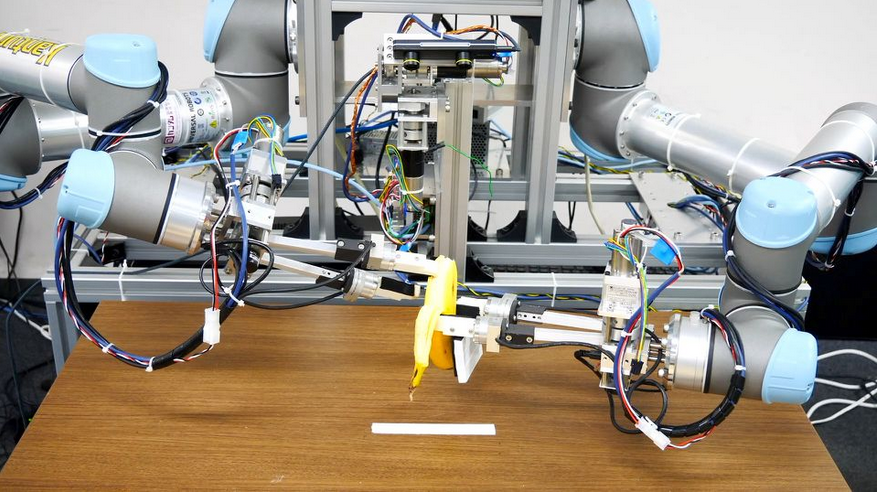
\includegraphics[height=4cm]{./figure/banana.png}
  \caption{双腕アームのロボットがバナナの皮を剥く様子}
  \end{center}
 \end{figure}

\subsection{Interactive Imitation Learning}
また、IIL(Interactive Imitation Learning)と呼ばれる, ロボットの実行中に間欠的に人間からフィードバックを受け取り、ロボットの振る舞いをオンラインで改善するための模倣学習(IL)の手法も発展しており、自動運転やロボットアームのマニピュレーション等様々なタスクで用いられている\cite{iil}
\begin{figure}[htbp]
 \begin{center}
 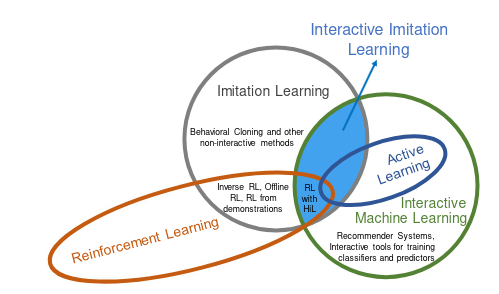
\includegraphics[height=4cm]{./figure/iil.png}
 \caption{IILの概要}
 \end{center}
\end{figure}

だが、異なる種類のフィードバックを組み合わせる方法や、ユーザーのフィードバックを同じ学習ポリシーの中にシームレスに入れることは現在の方法では難しく、データセットを組み合わせたり情報抽出時の工夫などが必要である. 


\section{参考文献}

\begin{thebibliography}{99H}
\bibitem{dqn} Volodymyr Mnih, Koray Kavukcuoglu, David Silver, Alex Graves, Ioannis Antonoglou, Daan Wierstra, and Martin Riedmiller. "Playing Atari with Deep Reinforcement Learning". NeurIPS, 2013
\bibitem{dqnrobot}Zhang F, Leitner J, Milford M, "Upcroft B and Corke P Towards vision-based deep reinforcement learning for robotic motion control" 2015
\bibitem{naf} Shixiang Gu, Timothy Lillicrap, Ilya Sutskever, and Sergey Levine. "Continuous Deep Q-Learning with Model-based Acceleration". ICML, 2016
\bibitem{NAFdrone} Regulariging Action Policies for Smooth Control with Reinforcement Learning, Siddharth Mysore, Bassel Mabsout, Renato Mancuso, Kate Saenko, 2021
\bibitem{ddqn} Hado van Hasselt, Arthur Guez, and David Silver. "Deep Reinforcement Learning with Double Q-Learning". AAAI, 2016
\bibitem{gps} End to End Training of Deep Visuomotor Policies, Sergey Levine, Chelsea Finn, Trevor Darrell, Pieter Abbeel, 2016
\bibitem{gorilla}Arun Nair, Praveen Srinivasan, Sam Blackwell, Cagdas Alcicek, Rory Fearon, Alessandro De Maria, Vedavyas Panneershelvam, Mustafa Suleyman, Charles Beattie, Stig Petersen, Shane Legg, Volodymyr Mnih, Koray Kavukcuoglu, and David Silver. "Massively Parallel Methods for Deep Reinforcement Learning". ICML, 2015
\bibitem{gpsTensegrity} Deep Reinforcement Learning for Tensegrity Robot Locomotion, Marvin Zhang, Xinyang Geng, Jonathan Bruce, Ken Caluwaerts, Massimo Vespignani, Vytas SunSpiral, Pieter Abbeel, Sergey Levine, 2017
\bibitem{rainbow} Matteo Hessel, Joseph Modayil, Hado van Hasselt, Tom Schaul, Georg Ostrovski, Will Dabney, Dan Horgan, Bilal Piot, Mohammad Azar, and David Silver. "Rainbow: Combining Improvements in Deep Reinforcement Learning". AAAI, 2018
\bibitem{agent57} Adrià Puigdomènech Badia, Bilal Piot, Steven Kapturowski, Pablo Sprechmann, Alex Vitvitskyi, Daniel Guo, and Charles Blundell. "Agent57: Outperforming the Atari Human Benchmark". ICML, 2020
\bibitem{r2d2} Steven Kapturowski, Georg Ostrovski, John Quan, Remi Munos, and Will Dabney. "Recurrent Experience Replay in Distributed Reinforcement Learning". ICLR, 2019.
\bibitem{r2d3} Tom Le Paine, Caglar Gulcehre, Bobak Shahriari, Misha Denil, Matt Hoffman, Hubert Soyer, Richard Tanburn, Steven Kapturowski, Neil Rabinowitz, Duncan Williams, Gabriel Barth-Maron, Ziyu Wang, Nando de Freitas, and Worlds Team. "Making Efficient Use of Demonstrations to Solve Hard Exploration Problems". ICLR, 2020
\bibitem{regularizing} Regularizing Action Policies for Smooth Control with Reinforcement Learning, Siddharth Mysore, Bassel Mabsout, Renato Mancuso, Kate Saenko, 2021
\bibitem{ac} "Actor-Critic Reinforcement Learning for Control with Stability Guarantee", Minghao Han, Lixian Zhang, Jun Wang, Wei Pan, 2020
\bibitem{sac} "Soft Actor-Critic: Off-Policy Maximum Entropy Deep Reinforcement Learning with a Stochastic Actor", Tuomas Haarnoja, Aurick Zhou, Pieter Abbeel, Sergey Levine, 2018
\bibitem{mujika} "Multi-task learning with deep model based reinforcement learning, Asier Mujika", 2017
\bibitem{meiro} "Piotr Mirowski, Razvan Pascanu, Fabio Viola, Hubert Soyer, Andrew J. Ballard, Andrea Banino, Misha Denil, Ross Goroshin, Laurent Sifre, Koray Kavukcuoglu, Dharshan Kumaran, Raia Hadsell, Learning to Navigate in Complex Environments", 2017
\bibitem{coberl} CoBERL: Contrastive BERT for Reinforcement Learning, Andrea Banino, Adrià Puidomenech Badia, Jacob Walker, Tim Scholtes, Jovana Mitrovic, Charles Blundell, 2022
\bibitem{banana} Heecheol Kim, Yoshiyuki Ohmura, and Yasuo Kuniyoshi. "Robot peels banana with goal-conditioned dual-action deep imitation learning". arXiv preprint arXiv:2203.09749, 2022.
\bibitem{iil}Interactive Imitation Learning in Robotics: A Survey, Carlos Celemin, Rodrigo Pérez-Dattari, Eugenio Chisari, Giovanni Franzese, Leandro de Souza Rosa, Ravi Prakash, Zlatan Ajanović, Marta Ferraz, Abhinav Valada, Jens Kober, 2022

\end{thebibliography}

\end{document}
